\documentclass[runningheads,a4paper]{llncs}
\usepackage{amssymb}
\setcounter{tocdepth}{3}
\usepackage{listings}
\usepackage{booktabs}
\usepackage{mathtools}
\usepackage{tabularx}
\usepackage{fixltx2e}
\usepackage[hyphens]{url}
\usepackage{hyperref}
\usepackage{upquote,textcomp}
\lstset{breaklines=true, basicstyle=\scriptsize\ttfamily, upquote=true}

\usepackage{fancyvrb}
\VerbatimFootnotes
\usepackage{cprotect}

\usepackage{graphicx}
\makeatletter
\def\maxwidth#1{\ifdim\Gin@nat@width>#1 #1\else\Gin@nat@width\fi}
\makeatother

\usepackage{amsmath}
\usepackage{color,graphics,array,csscolor}
\usepackage{pmml-new}

\usepackage{fontspec,unicode-math}
\usepackage[Latin,Greek]{ucharclasses}
\setTransitionsForGreek{\fontspec{Times New Roman}}{}

\usepackage{subscript}
\lstset{breaklines=true, basicstyle=\scriptsize\ttfamily}

\usepackage[margin=1.72in]{geometry}

\begin{document}
\mainmatter

\title{Jailbreaking your reference lists:\\ OpenCitations strike again}
\titlerunning{Jailbreaking your reference lists}
\author{Silvio Peroni\inst{1} \and
David Shotton\inst{2} \and
Fabio Vitali\inst{1}}
\authorrunning{Silvio Peroni et al.}
\institute{DASPLab, DISI, University of Bologna, Bologna, Italy\and
Oxford e-Research Centre, University of Oxford, Oxford, UK\\
\email{silvio.peroni@unibo.it, 
david.shotton@oerc.ox.ac.uk, 
fabio.vitali@unibo.it}}
\maketitle

\begin{abstract}
In this poster paper we provide an overview of the OpenCitations Project (\url{http://opencitations.net}) and of its main outcome, the OpenCitations Corpus, which is an open repository of scholarly citation data made available under a CC0 license, providing in RDF accurate citation information harvested from the scholarly literature, starting from the PubMed Central OA subset.

{\bf RASH:} \url{https://w3id.org/oc/paper/occ-poster-iswc2016.html}

\keywords{Citation Database, OpenCitations, OpenCitations Corpus, Scholarly Communication, Semantic Publishing}
\end{abstract}


\section{Introduction}

Reference lists from academic articles are the core elements of scholarly communication, since they both permit the attribution of credit and integrate our independent research endeavours. But the cruel reality is that they are not freely available. For instance, UK research universities each pay tens of thousands of pounds annually  \cite{__RefNumPara__293_1852566440} for accessing to commercial sources of scholarly citations -- Scopus and Web of Science. In the current age where Open Access is considered a necessary practice in research, it is a scandal that reference lists from journal articles are not readily and freely available for use by all scholars. As we have already stated in a previous work  \cite{__RefNumPara__293_1852566440}: 

\begin{quote}
Citation data now needs to be recognized as a part of the Commons -- those works that are freely and legally available for sharing -- and placed in an open repository, where they should be stored in appropriate machine-readable formats so as to be easily reused by machines to assist people in producing novel services.
\end{quote}

This is the main premise behind the OpenCitations Project and a number of other complementary initiatives including Semantic Lancet\footnote{\url{http://semanticlancet.eu/}} \cite{__RefNumPara__69_1852566440}, Springer LOD\footnote{\url{http://lod.springer.com/}}, OpenAIRE\footnote{\url{https://www.openaire.eu/}} \cite{__RefNumPara__71_1852566440} and Scholarly Data\footnote{\url{http://www.scholarlydata.org/}} \cite{__RefNumPara__75_1852566440}. Since the beginning of July, OpenCitations has started to ingest and process the reference lists of scholarly papers available in Europe PubMed Central\footnote{\url{http://europepmc.org/}}. In this paper we provide a brief overview of its main components that make the extraction and description of such reference lists in RDF possible.

\section{OpenCitations and its Corpus}

The OpenCitations Project (\url{http://opencitations.net}) is creating an open dataset of citation data integrated with a SPARQL endpoint\footnote{\url{https://w3id.org/oc/sparql}} and a very simple Web interface that shows only the data about bibliographic entities\footnote{Additional and more user-friendly interfaces will be available in the coming months, and will be described in the project homepage.}. Its main output is the Open Citations Corpus (OCC), an open repository of scholarly citation data made available under a Creative Commons CC0 license\footnote{\url{https://creativecommons.org/publicdomain/zero/1.0/legalcode}}, which provides accurate bibliographic references harvested from the scholarly literature, described using the SPAR Ontologies\footnote{\url{http://www.sparontologies.net/}} \cite{__RefNumPara__17_1852566440} according to the OCC metadata document  \cite{__RefNumPara__19_1852566440}, that others may freely build upon, enhance and reuse for any purpose, without restriction under copyright or database law.

The OCC stores metadata relevant to these citations in RDF, encoded as JSON-LD, and makes them available through a SPARQL endpoint (and, in the near future, as downloadable datasets). It includes information about six different kinds of bibliographic entity:
\begin{itemize}
\item {\bf bibliographic resources} (br) -- resources that cite/are cited by other bibliographic resources (e.g. journal articles), or that contain such citing/cited resources (e.g. journals);
\item {\bf resource embodiments} (re) -- details of the physical or digital forms in which the bibliographic resources are made available by their publishers;
\item {\bf bibliographic entries} (be) -- the literal textual bibliographic entries occurring in the reference lists within bibliographic resources, that reference other bibliographic resources;
\item {\bf responsible agents} (ra) -- names of agents having certain roles with respect to bibliographic resources (i.e. names of authors, editors, publishers, etc.);
\item {\bf agent roles} (ar) -- roles held by agents with respect to bibliographic resources (e.g. author, editor, publisher);
\item {\bf identifiers} (id) -- external identifiers (e.g. DOI, ORCID, PubMedID) associated with the bibliographic entities.
\end{itemize}

The corpus URL (\url{https://w3id.org/oc/corpus/}) identifies the entire OCC, which is composed of several sub-datasets, one for each of the aforementioned bibliographic entities included in the corpus. Each of these has a URL composed by suffixing the corpus URL with the two-letter short name for the class of entity (e.g. ``be'' for a bibliographic entry) followed by an oblique slash (e.g. \url{https://w3id.org/oc/corpus/be/}). Each dataset is described appropriately by means of the Data Catalog Vocabulary\footnote{\url{https://www.w3.org/TR/vocab-dcat/}} and the VoID Vocabulary\footnote{\url{https://www.w3.org/TR/void/}}.

Upon initial curation into the OCC, a URL is assigned to each entity within each sub-dataset, all of which can be accessed in different formats (HTML, RDF/XML, Turtle, and JSON-LD) via content negotiation. Each entity URL is composed by suffixing the sub-dataset URL with a number assigned to each resource, unique among resources of the same type, which increments for each new entry in that resource class. For instance, the resource \url{https://w3id.org/oc/corpus/be/537} is the 537\textsuperscript{th} bibliographic entry recorded within the OCC. Each of these entities has associated metadata describing its provenance by means of PROV-O\footnote{\url{https://www.w3.org/TR/prov-o/}} and its PROV-DC extension\footnote{\url{https://www.w3.org/TR/prov-dc/}} (e.g. \url{https://w3id.org/oc/corpus/be/537/prov/se/1}). In particular, we keep track of the curatorial activities related to each OCC entity, the curatorial agents involved, and their roles. Additional information about OCC's handling of citation the data, and the way they are represented in RDF, are detailed in the official OCC Metadata Document  \cite{__RefNumPara__19_1852566440}.

The ingestion of citation data into the OCC is handled by two Python scripts called {\em Bibliographic Entries Extractor} ({\em BEE}) and the {\em SPAR Citation Indexer} ({\em SPACIN}), available in the OCC's GitHub repository\footnote{\url{https://github.com/essepuntato/opencitations}}. As shown Fig.~\ref{refIllustration0}, BEE is responsible for the creation of JSON files containing information about the XML articles in the OA subset of PubMed Central (retrieved by using the Europe PubMed Central API\footnote{\url{https://europepmc.org/RestfulWebService}} and used as input data). Each of these JSON files also includes the complete reference list of the paper under consideration extracted by means of XPath queries. Then, SPACIN processes each JSON file, retrieves metadata information about all the citing/cited articles described in it by querying the Crossref API\footnote{\url{http://api.crossref.org/}} and the ORCID API\footnote{\url{http://members.orcid.org/api/}}, and stores all the generated RDF resources in the file system in JSON-LD format and within the OCC triplestore, disambiguating the resources that have been added previously by means of the retrieved identifiers (i.e. DOI, PMID, PMCID, ORCID, URL). It is worth noting that the triplestore includes all the data about the curated entities except their provenance data and the descriptions of the datasets, that are accessible only via HTTP.

The workflow introduced in Fig.~\ref{refIllustration0} is a process that runs until no more JSON files can be produced by BEE. Thus, the current instance of the OCC is evolving dynamically in time, and can be easily extended so as to interact with additional REST APIs from different sources, so as to gather additional article metadata and their related references. Currently, each day the workflow adds about 2 million triples to the corpus, describing more than 20,000 new citing/cited bibliographic resources and about 100,000 new authors, about 5\% of whom are disambiguated through their ORCID ids.
\begin{figure}[h!]
\centering
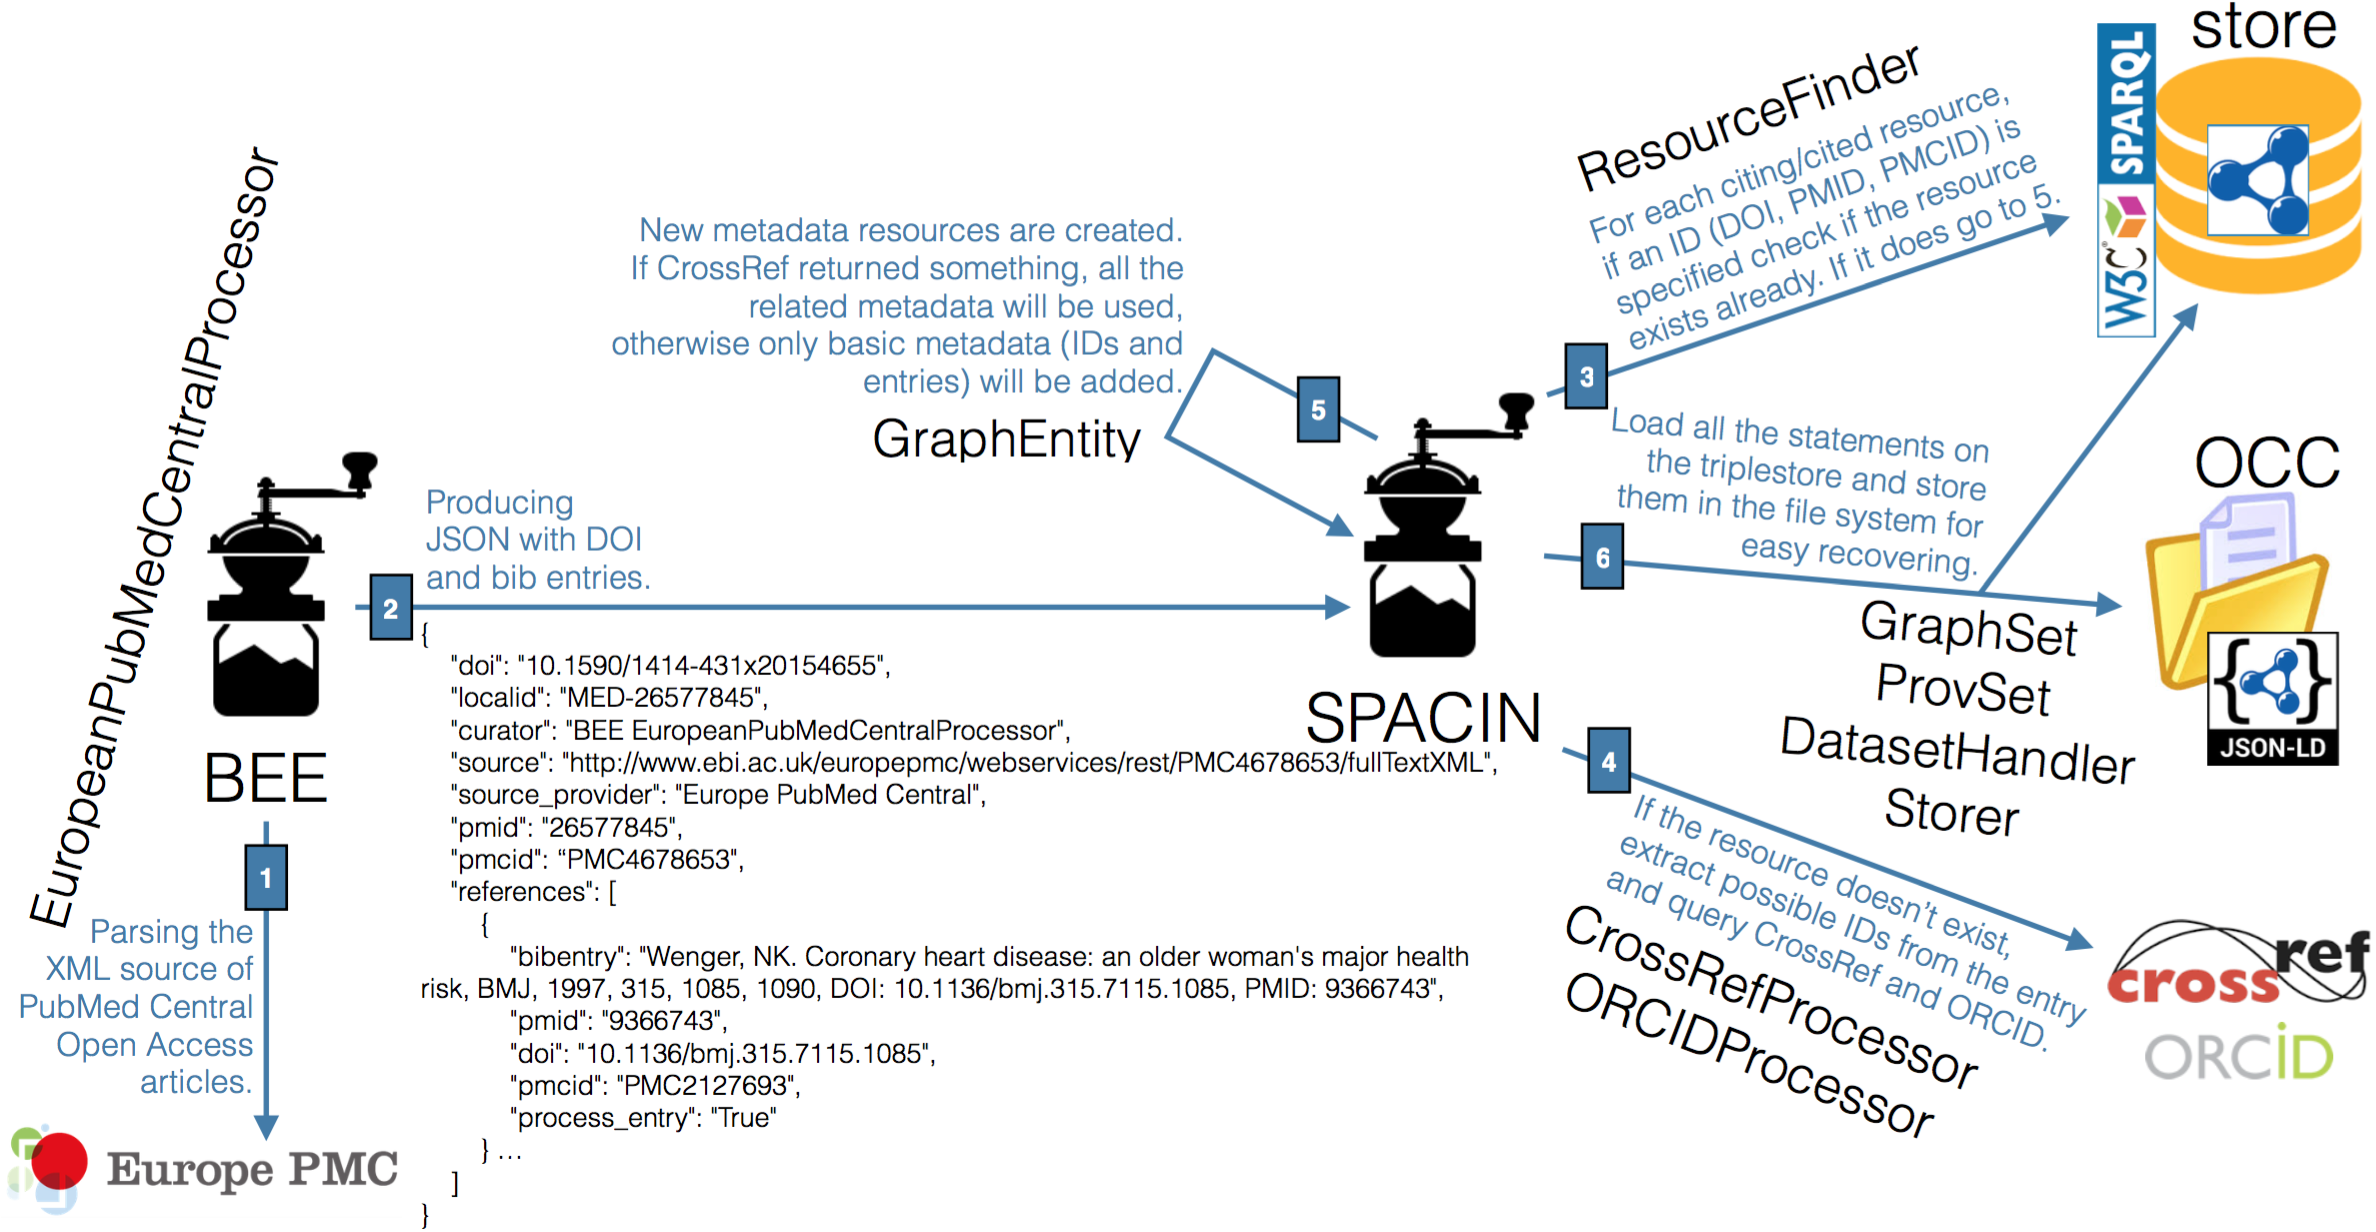
\includegraphics[width=\maxwidth{\textwidth}]{img/1000020100000948000004D0192123CB.png}
\cprotect\caption{The steps involving BEE and SPACIN, and their related Python classes, in the production of the OpenCitations Corpus.}
\label{refIllustration0}
\end{figure}


\section{Conclusions}

In this poster paper we have introduced the OpenCitations Project, which is involved in creating an open repository of accurate bibliographic references harvested from the scholarly literature: the OpenCitations Corpus (OCC). The new instance of the OCC has just been established, and already includes 728,991 citation links (as of August 30, 2016) -- a number that will grow quickly over the coming months as the continuous workflow adds new data dynamically from Europe PubMed Central and other authoritative sources. The OCC SPARQL endpoint is presently available for use, and distributions of the OCC will shortly be made openly available for bulk download -- the first of these by early September 2016, with subsequent incremental additions.

We are currently working on two different aspects. First of all, we are developing tools for linking the resources within the OCC with those included in other datasets, e.g. Scholarly Data. In addition, we are experimenting with the use of multiple parallel instantiations of SPACIN, so as to increase the amount of new information that can be processed daily. 

\begin{thebibliography}{4}

\bibitem{__RefNumPara__71_1852566440} Alexiou, G., Vahdati, S., Lange, C., Papastefanatos G., Lohmann, S. (2016). OpenAIRE LOD services: Scholarly Communication Data as Linked Data. To appear in Proceedings of SAVE-SD 2016. \url{http://cs.unibo.it/save-sd/2016/papers/html/alexiou-savesd2016.html}
\bibitem{__RefNumPara__69_1852566440} Bagnacani, A., Ciancarini, P., Di Iorio, A., Nuzzolese, A. G., Peroni, S., Vitali, F. (2014). The Semantic Lancet Project: A Linked Open Dataset for Scholarly Publishing. In EKAW 2014 Satellite Events: 101--105. \url{http://dx.doi.org/10.1007/978-3-319-17966-7\_10}
\bibitem{__RefNumPara__75_1852566440} Nuzzolese, A. G., Gentile, A. L., Presutti, V., Gangemi, A. (2016). Conference Linked Data -- Our Web Dog Food has gone gourmet. To appear in Proceedings of ISWC 2016.
\bibitem{__RefNumPara__17_1852566440} Peroni, S. (2014). The Semantic Publishing and Referencing Ontologies. In Semantic Web Technologies and Legal Scholarly Publishing: 121--193. \url{http://dx.doi.org/10.1007/978-3-319-04777-5\_5}
\bibitem{__RefNumPara__293_1852566440} Peroni, S., Dutton, A., Gray, T., Shotton, D. (2015). Setting our bibliographic references free: towards open citation data. Journal of Documentation, 71 (2): 253--277. \url{http://dx.doi.org/10.1108/JD-12-2013-0166}
\bibitem{__RefNumPara__19_1852566440} Peroni, S., Shotton, D. (2016). Metadata for the OpenCitations Corpus. figshare. \url{https://dx.doi.org/10.6084/m9.figshare.3443876}

\end{thebibliography}

\end{document}